\section{Introduction}
GPGPU (General-purpose computing on graphics processing units) have been on the
rise, due to limitations on CPUs, such as power consumption, and the fact
that the computational potential of GPUs (Graphical processing unit) is vastly
superior to CPUs, as seen in Figure \ref{potential}. There are technical and physical
issue in reaching this potential, for example memory bandwidth bottle-necking computation, but there is
also the conceptual issue of how to map parallelism to parallel hardware.
\begin{figure}[h]
	\centering
	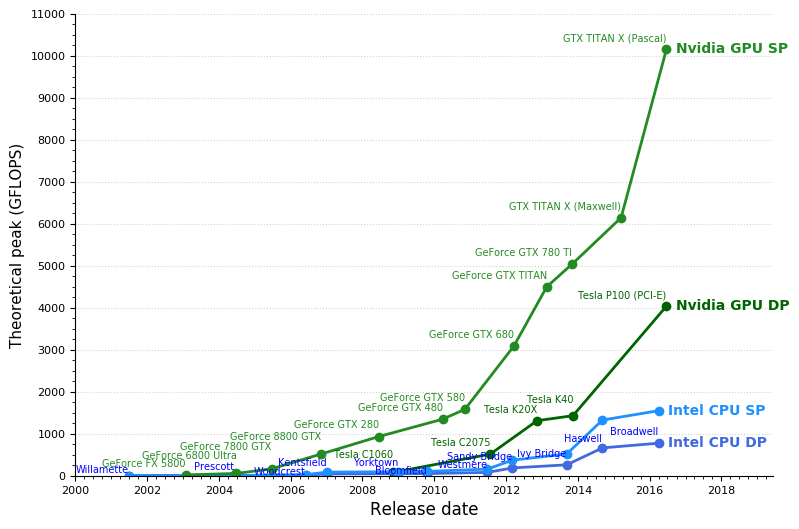
\includegraphics[width=.8\textwidth]{resources/graf.png}
	\caption{A graph showing the computational potential of CPUs and GPUs from 2000---2016 \cite{cpu-vs-gpu}}
	\label{potential}
\end{figure}

In this project we will implement an autotuner for the programming language
Futhark \cite{futhark-home}, which is an ongoing research project at The University of Copenhagen. Futhark is a statically typed, data-parallel, and
purely functional array language. The aim of Futhark is to shift the burden of
writing efficient parallel code from the programmer to the compiler. The
burden referred to is the requirement for a deep understanding of GPU hardware architecture and compiler knowledge for the language used, which is necessary to write efficient GPU code. Even when this requirements is met, using common GPU languages such as CUDA and OpenCL will still result in non-portable code as a lot of the optimizations made
are specific to a certain GPU, or at least to a certain GPU architecture. 

\begin{figure}
\centering
\lstset{language=haskell}
\begin{lstlisting}
let dotprod [n] (xs: [n]f32) (ys: [n]f32): f32 =
reduce (+) 0f32 (map2 (*) xs ys)

let main [n][m][p] (xss: [n][m]f32) (yss: [m][p]f32): [n][p]f32 =
map (\xs -> map (dotprod xs) (transpose yss)) xss
\end{lstlisting}%
\captionof{lstlisting}{Matrix-matrix multiplication in Futhark \cite{ppopp}}
\label{IntromatmultFuthark}
\end{figure}
A Futhark program for matrix-matrix multiplication can be seen in listing
\ref{IntromatmultFuthark}. The syntax is similar to languages such as ML and
Haskell. It is a good example of how Futhark differs from CUDA or OpenCL (we
would have included an example of CUDA, but it was too long, it can be found in Appendix
\ref{cuda-matmult}). It should be clear why, if Futhark has the possibility to
achieve speeds similar to those of CUDA and OpenCL Futhark would be very
preferable.

To achieve the shift in burden from programmer to compiler, the Futhark
compiler creates multiple semantically equivalent parallelisations, called code
versions, for each parallel construct. The code versions are combined into
a single program where the semantically equivalent code versions are guarded
by a run-time comparison, so that only a single one of them are executed and the
semantics of the new program is equivalent to the original Futhark program. 
The comparisons are between a user defined parameters and values that are
a reflection of the input size.

Adjusting these parameters to select the execution that will minimize the
running time is called tuning. The aim of this project is to automatize this
process, so that it does not have to be done by hand. This is what we
call autotuning. To find the optimal set of values for the parameters our
autotuner is going to perform an exhaustive search, that means trying out every
meaningful set of values and select the best one. 
%this is added
We perform an exhaustive search
due to the suspicion that Futhark programs are relatively small, and therefore 
an exhaustive search might be a feasible solution.

The remainder of this report is structured as follows. In section \ref{BabyGotBack} 
we present what parallelism is and the concepts behind how Futhark transforms functional 
code into efficient parallel code, 
% denne sæting er svær
as well as presenting the structure of what in Futhark that is to be autotune. 
In section \ref{imp} we explore how we have implemented the exhaustive autotuner along
with thoughts about future concerns the autotuner may face, due to Futhark being an
ongoing project. We evaluate the autotuner in section \ref{GottaGoFast} in order to see the
feasibility of the exhaustive autotuner. We have then reflected
on the results achieve, and suggested improvements in section \ref{synData}. 

\begin{comment}
Tuning Futhark, is like being a kid in a candy store. We have a bag
(parallel hardware, usually a GPU), that is to be filled
with candy (parallelism in a program). We have a priority of the candy we want, 
for example we only want the licorice, if we also get the gummy (guards). We want to 
efficiently pack the bag in order to get as much candy as possible. If we
overpack the bag, it will get too heavy (introducing overhead larger than gain)
and it will take longer to get the bag home. If we underfill we will
obviously get less candy. So the only way to know how much candy we can get is to check,
for each bag that we use, how much candy will fit in it, for some bags we will only have 
room for a piece of gummy, while others will have room for the gummy and licorice. Therefore
we try every combination of candy, while still respecting the priority 
(tuning the parameters). 
\end{comment}


